% !TEX root = autopaxos.tex
% !TEX TS-program = pdflatexmk
% For TeXShop on OS X and Herbert Schulz's latexmk engine.

\section{Evaluation}\label{evaluation}

\subsection{Measurement}
Our first task was to quantify the amount and character of information at our disposal.
After we wrapped all of the appropriate calls in instrumentation, we created a pair of experiments which set random environment constraints and then evaluated how accurately the system tracked those values.

% RTT tracking
\begin{figure}[htbp]
\begin{center}
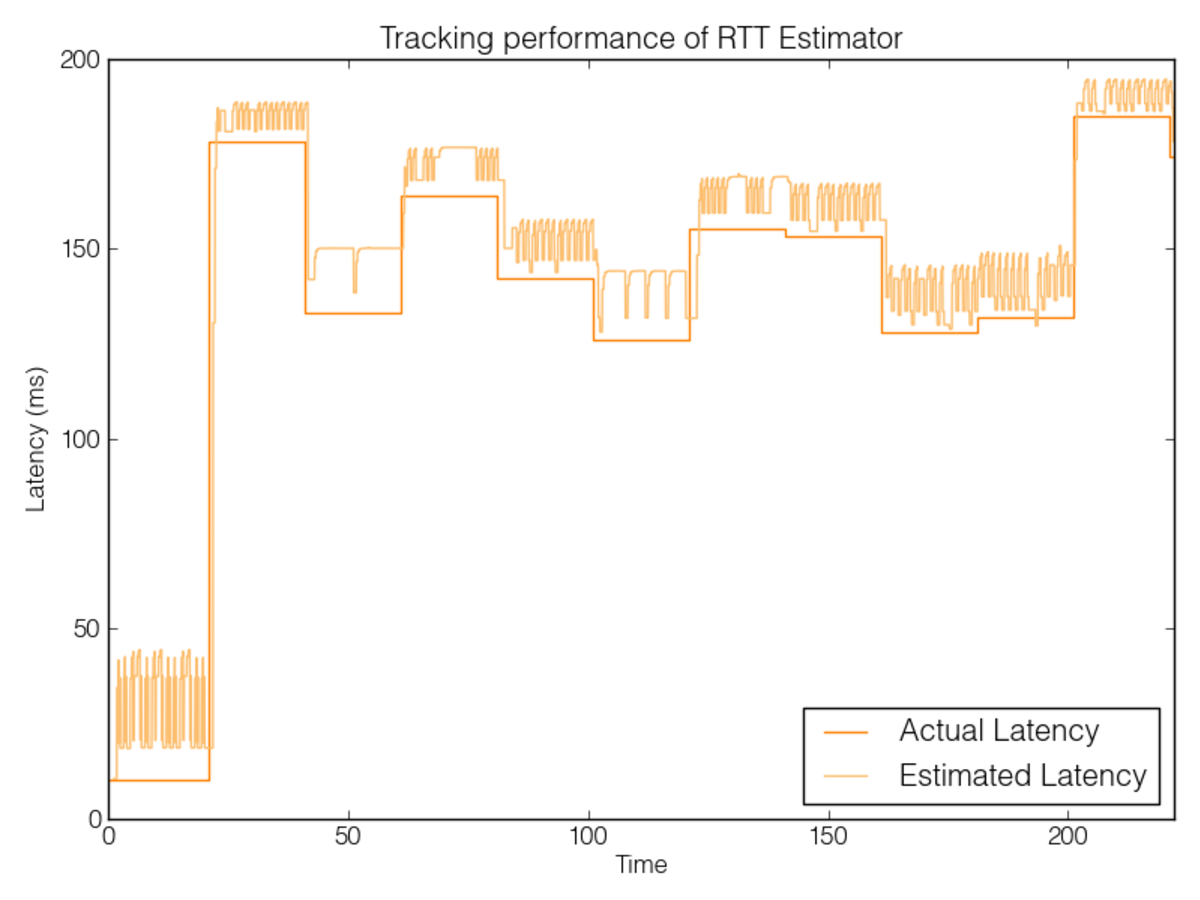
\includegraphics[width=\columnwidth]{track_rtt_final}
\caption{Estimation of latency.}
\label{track_rtt}
\end{center}
\end{figure}

Figure~\ref{track_rtt} shows the difference between the actual latency imposed on our library (simulated using a network wrapper) and the estimate that the system produces.
We use a simple, exponentially-weighted moving average (\ref{ewma}) to track and integrate the round-trip measurements.
\begin{equation}\label{ewma}
Y_n = (\alpha)x_n + (1-\alpha)Y_{n-1}
\end{equation}
Likewise, figure~\ref{track_mtbf} presents real and estimated values for mean-time-between-failure.
Our driver code called shutdown and recover hooks that we placed into the library at random intervals.
To measure MTBF, we store a small sliding window with the times of the last 10 recorded node drop events.
The estimated MTBF is simply the average of these differences.

% Drop tracking
\begin{figure}[htbp]
\begin{center}
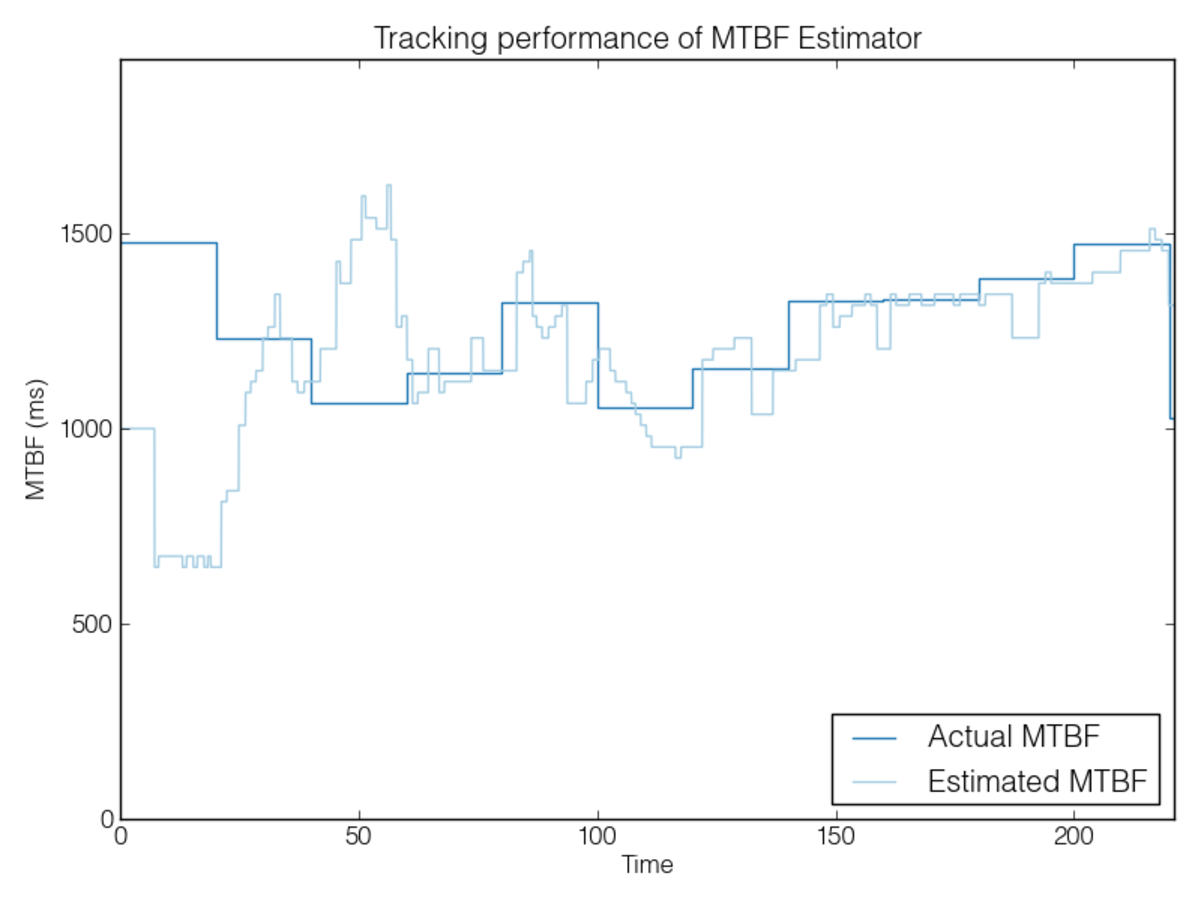
\includegraphics[width=\columnwidth]{track_mtbf_final}
\caption{Estimation of mean time between failure.}
\label{track_mtbf}
\end{center}
\end{figure}

While our latency tracker appears much more precise, this is due to the fact that our experiments were conducted on the same machine (and in point of fact, inside the same process address space).
Our MTBF estimator performs well enough after a burn-in phase---a result of using an un-seeded sliding average.

\subsection{Policy}
Once our data has been gathered, we compute the cost metric presented before from our estimates.
Figure~\ref{track_policy} shows the transitive effects that the errors from our input estimators have on our cost model.
A reasonably stable cost metric is important for maintaining steady-state behavior, and while there are some estimation artifacts (likely due to message pile-up), our estimation is sufficient for our purposes.

% analytical model
\begin{figure}[htbp]
\begin{center}
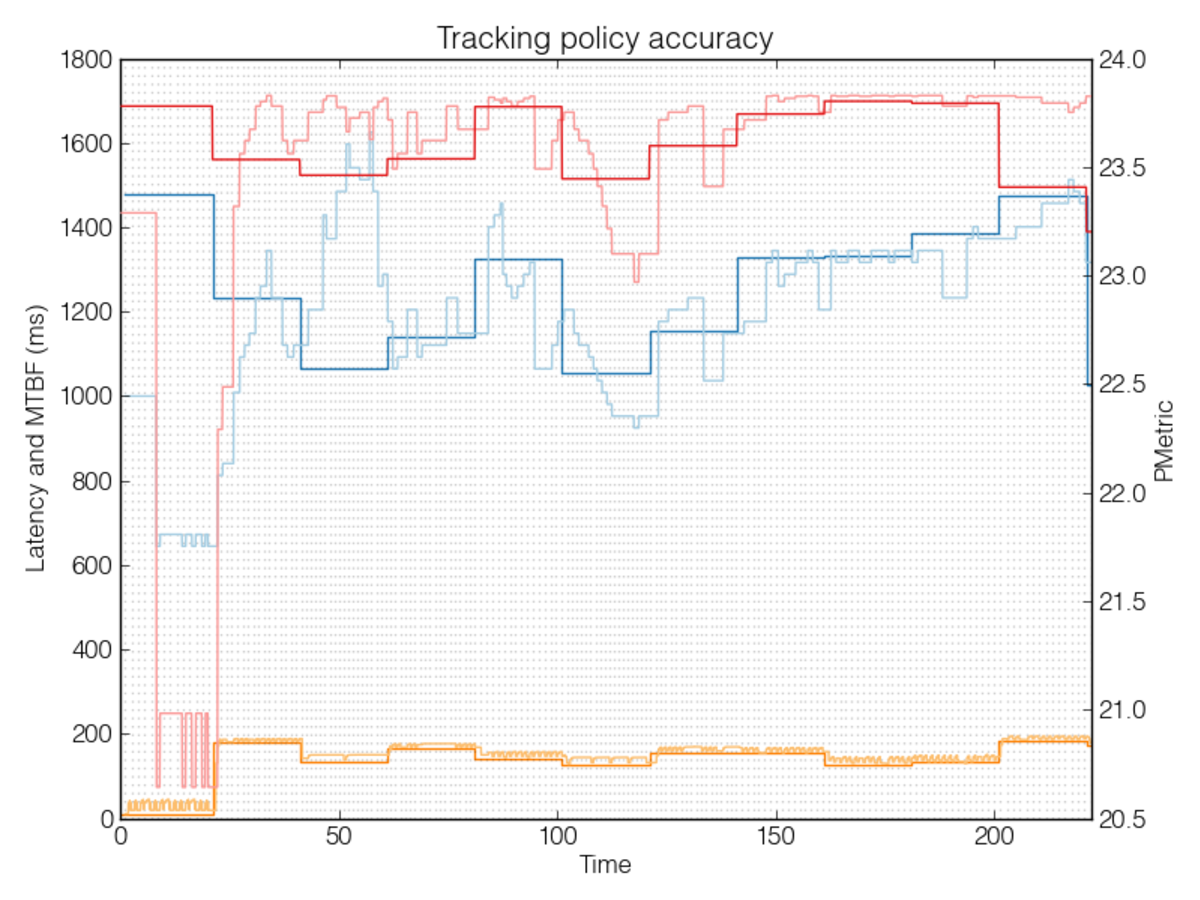
\includegraphics[width=\columnwidth]{track_policy_final}
\caption{Latency tracking is at bottom, in orange, MTBF tracking is in the middle in blue, and the resulting estimate for goodness (PMetric) is shown at top as the light red line. The dark red line represents the same calculation, but computed using exact (oracle) numbers, for reference.}
\label{track_policy}
\end{center}
\end{figure}

The other half of our policy model is a brute-force search algorithm.
In order to identify the best combination of tuning parameters, we exhaustively sweep the parameter space and identify the global maximum (in terms of our estimated PMetric score).
Figure~\ref{search_space} displays a set of parameter curves in this search space.
Here, we are iterating over the node timeout value ($\Tto$) and the heartbeat interval ($\Thb$).
The takeaway here is that while nonlinear, the search space is surprisingly smooth, and (as we describe below), somewhat devoid of saddle points or local maxima.

% parameters
\begin{figure}[htbp]
\begin{center}
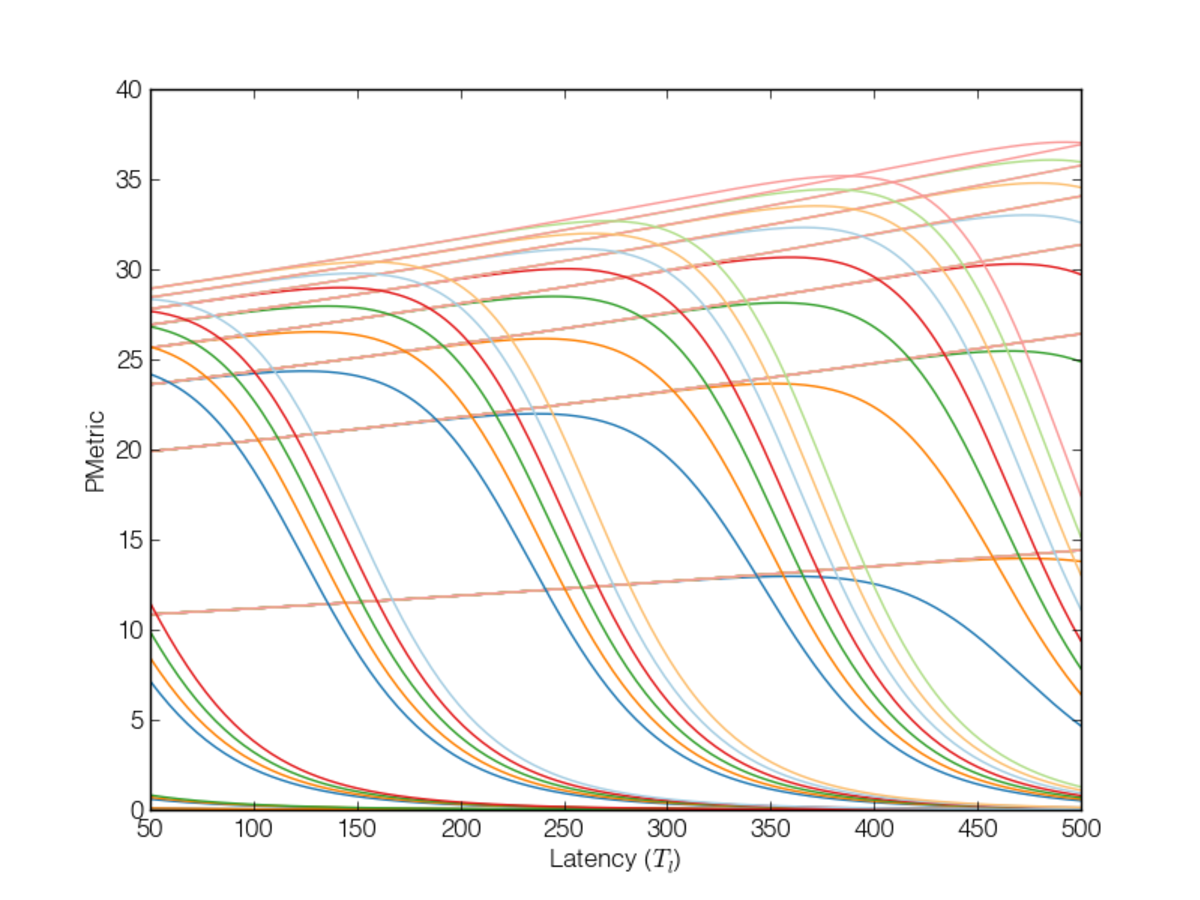
\includegraphics[width=\columnwidth]{search_space_final}
\caption{A 2-dimensional search space.}
\label{search_space}
\end{center}
\end{figure}

\subsection{Tuning}
% monotonic shift
In order to evaluate efficacy of our policy model in improving the performance of our Paxos System, we subjected the Paxos System to a environment with a monotonically increasing latency (Figure~\ref{monotonic_shift}).  As latency of the network increases with time, the Goodness of the network accordingly decreases.  We hypothesized that as the network becomes worse, the non-adjusting Paxos system would continue to worsen in its goodness score as well while the autotuning one would be relatively unaffected, yet here we observe the opposite suggesting that the changes that \emph{Autopaxos} is making to its parameters is actually hurting its performance. 

\begin{figure}[htbp]
\begin{center}
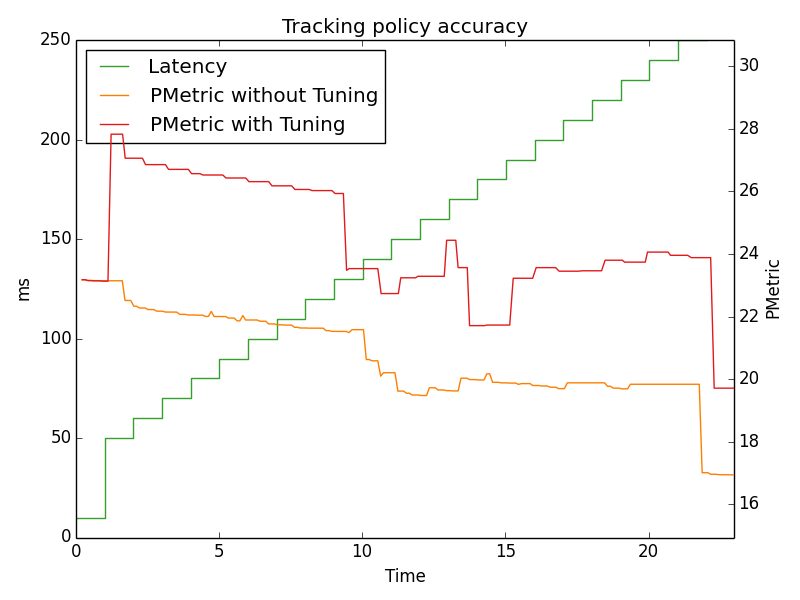
\includegraphics[width=\columnwidth]{monotonic_shift}
\caption{Monotonic Shift of Latency.  Goodness measures the actual $\frac{uptime}{traffic}$ of the system on the network.}
\label{monotonic_shift}
\end{center}
\end{figure}